\section{Extended experiments and recovered protocols}\label{app:extended}

\paragraph{Protocol.} Confirmatory thresholds follow the recovered pre-registrations. Freezing is audited experiment by experiment: E2 windowing changed after a one-image pilot, G1 predictors were proposed after seed1, and exploratory analyses are not promoted to confirmation. Images are from
DIV2K validation (0801--0812) unless stated; $R_b$ uses each recovered protocol: F1/G1/E3 average RGB to grayscale, L2 pools RGB channel energies, and E1/D11 retain RGB metrics.
Exploratory analyses are labelled as such.

%-------------------------------------------------------------------
\subsection{The mismatch cost is predictable (E2)}\label{sec:exp-e2}

\paragraph{Setup.} 12 DIV2K images, five tasks (single image $\times2$,
$\times4$; sparse pixels 10\%, 25\%, 50\%). In each of the three bands we
multiply the true spectrum by $\kappa\in\{1/16,1/4,4,16\}$, reconstruct with a
GP (linear), and measure the lost recoverability in that band, giving 60
cells \src{E2§2}. Band energies are computed after a Hann window on
both signal and error; the window was not specified in the pre-registration
and was added after a one-image run showed boundary leakage (single-image
$\times4$ $b_3$ measured $R=0.56$ at 0.004\% transmittance). After the fix,
single-image $\times4$ $b_2$ measures $R=0.085$ against an a-priori 0.08
\src{E2§1}. Only the metric changed, not hypotheses or criteria.

\begin{table}[t]\centering\small
\caption{Original E2 reported criteria (60 cells, 12-image means)
\src{E2§2; E4-T1}.}\label{tab:e2}
\begin{adjustbox}{max width=\linewidth}\begin{tabular}{lcc}\toprule
Criterion & Threshold & Result\\\midrule
a. Spearman(band-avg.\ prediction, measured) & $\ge0.8$ & \textbf{0.90}\\
b. $R<0.3$: over-est.\ $>$ under-est. & $\ge80\%$ & 4/4\\
b. $R>0.7$: under-est.\ $>$ over-est. & $\ge80\%$ & 6/7\\
c. median $|$pred.$-$meas.$|$ & $\le0.05$ & 0.038\\
d. Spearman(a-priori prediction, measured) & $\ge0.7$ & 0.79\\
\bottomrule\end{tabular}\end{adjustbox}
\end{table}

\begin{table}[t]\centering\small
\caption{Original E2 measured / band-averaged predicted cost $\Delta$ (fraction of band
energy) \src{E2§3}.}\label{tab:e2cells}
\setlength{\tabcolsep}{3pt}
\begin{adjustbox}{max width=\linewidth}\begin{tabular}{lccccc}\toprule
Task, band & $R$ & $\kappa{=}\tfrac1{16}$ & $\tfrac14$ & 4 & 16\\\midrule
SI$\times2$ $b_2$ & .80 & .230/.402 & .047/.101 & .067/.031 & .165/.056\\
SI$\times2$ $b_3$ & .11 & .084/.097 & .044/.058 & .194/.380 & \textbf{1.370}/2.648\\
SI$\times4$ $b_2$ & .085 & .060/.074 & .029/.045 & .150/.336 & \textbf{0.933}/2.590\\
Sparse 10\% $b_2$ & .37 & .197/.291 & .072/.144 & .110/.302 & .586/.976\\
Sparse 25\% $b_2$ & .70 & .226/.430 & .068/.139 & .094/.074 & .473/.149\\
Sparse 50\% $b_2$ & .90 & .148/.264 & .036/.046 & .024/.009 & .064/.015\\
\bottomrule\end{tabular}\end{adjustbox}
\end{table}

\paragraph{Independent reimplementation (E2r).} A separate implementation
reproduces all 60 aggregated cells from 12 images and five tasks. Its
post-hoc cost ranking is .902528, reference-prior ranking .797188 and
median absolute error .035099 (maximum 1.8895). Asymmetry counts are 4/4
and 6/7; all four frozen thresholds pass. These are distinct rerun numbers,
not replacements for individual original cells in Tables~\ref{tab:e2}
and~\ref{tab:e2cells}. The high maximum error limits quantitative
interpretation despite the passed median threshold \src{E2r}.

\paragraph{Results.} All four pre-registered criteria hold
(Table~\ref{tab:e2}). For example, single-image $\times4$ $b_2$ has under-estimation cost $.060$ and over-estimation cost $.933$ for reciprocal factors $1/16$ and $16$; the latter exceeds the matched recovery $.085$ and hence is worse than zero band reconstruction
(Table~\ref{tab:e2cells}). In high-$R$ bands the direction reverses. In the reported near-zero-recovery cell (single image $\times4$ $b_3$), both evaluated finite mismatch factors incur small costs; this is not uniform over arbitrarily large factors \src{E2§3}.
The band-averaged prediction over-estimates large-$\kappa$ costs in the reported examples; this direction is not general. For
decimation, evaluating Eq.~\eqref{eq:delta} per frequency with
Eq.~\eqref{eq:alias} and energy-weighting reduces approximation error in the reported exploratory calculation (exploratory:
Spearman 0.99, median error 0.004; e.g.\ SI$\times4$ $b_2$, $\kappa=4$:
predicted 0.151, measured 0.150) \src{E2§4}.
The single counter-example to the asymmetry is sparse 10\% $b_1$ ($R=0.92$;
under 0.072 vs.\ over 0.110): random sampling spreads aliasing across bands,
outside the scalar model \src{E2§2}.

%-------------------------------------------------------------------
\subsection{Low-reference-recovery bands: similarities among evaluated ASISR decoders (M2, E3)}\label{sec:exp-c}

\paragraph{Setup.} We compare four trained decoders that share the
EDSR-baseline encoder and the LIIF training protocol (DIV2K, 1000 epochs,
scale range $\times1$--$\times4$, seed 1): LIIF, LTE, SC-INR-eq and
SC-INR without the sinc footprint readout. This early comparison is not a matched SC-INR/NoSinc ablation; the latter is evaluated separately in F1/G1
against two linear references, LMMSE with the generic spectrum and LMMSE with
the image's own (oracle) spectrum, on $256^2$ centre crops of the first 30
images of Set14, BSD100 and Urban100 \src{OUT7.1/h6c}.

\begin{table}[t]\centering\small
\caption{Single image $\times4$, $R_b$ measured on data
\src{OUT7.1/h6c}. Regime by $\Rlin$: $b_2$, $b_3$ are C. gen./orac.: LMMSE with generic/oracle spectrum; SC-eq/SC-ns: SC-INR-eq / SC-INR-nosinc.}
\label{tab:h6c}
\setlength{\tabcolsep}{3pt}
\begin{adjustbox}{max width=\linewidth}\begin{tabular}{llcccccc}\toprule
Set & band & gen. & orac. & LIIF & LTE & SC-eq & SC-ns\\\midrule
Set14 & $b_2$ & .16 & .25 & .56 & .57 & .57 & .56\\
 & $b_3$ & .09 & .09 & .20 & .20 & .20 & .18\\
BSD100 & $b_2$ & .13 & .22 & .38 & .38 & .38 & .38\\
 & $b_3$ & .06 & .06 & .13 & .13 & .13 & .11\\
Urban100 & $b_2$ & .11 & .27 & .50 & .50 & .51 & .51\\
 & $b_3$ & .02 & .03 & .14 & .14 & .15 & .13\\
\bottomrule\end{tabular}\end{adjustbox}
\end{table}

\paragraph{$\times4$.} In both regime-C bands the trained networks recover
more than the evaluated oracle-periodogram linear reference: 0.38--0.57 vs.\ 0.22--0.27 in $b_2$
(1.7--2.3$\times$) and 0.13--0.20 vs.\ 0.03--0.09 in $b_3$ (2--6$\times$)
(Table~\ref{tab:h6c}). This comparison is consistent with benefits from a learned prior, but does not prove that all linear models or all alternative priors fail on these images.
The four decoders differ by at most 0.02 in either band.

\paragraph{Across scale factors (E3).} We repeat the measurement at
$\times2$, $\times3$, $\times8$ (27 cells: 3 scales $\times$ 3 bands $\times$
3 datasets) with the same networks; $\times8$ is out of the training range
\src{E3}. Pre-registered results (Table~\ref{tab:e3}): the a-priori
$\Rlin$ ranks the measured generic-LMMSE recovery with Spearman 0.952; in
10/12 regime-C cells all four networks exceed the oracle LMMSE and differ by
at most 0.03; in 9/9 regime-A cells the best network is within 0.05 of the
oracle LMMSE (largest gap $+0.016$); generic-LMMSE recovery decreases
monotonically with scale in 9/9 band--dataset pairs. The descriptive reference labels change with scale: $b_2$ is A at $\times2$ ($\Rlin=0.92$), B at $\times3$ (0.42) and
C at $\times8$ (0.011); $b_1$ enters B at $\times8$ (0.79)
\src{E3-key}. In all 12 C cells every network exceeds the oracle
(by $+0.002$ to $+0.244$) \src{E4-T2}.

\paragraph{Scale collapse (L1, pre-registered).} The measurement hypothesis is that recovery is more consistent across scales when frequency is expressed relative to LR Nyquist, $u=2s\nu$, than in absolute frequency; this comparison does not identify an observation-only causal limit. On
$240^2$ crops of the first 30 images per dataset, we measure $R(u)$ in seven
$u$ bins at $\times2/\times3/\times4$ for LIIF, LTE and SC-INR (seed 1) and
take the median range across scales, $D_{\mathrm{in}}$ \src{L1L2}. The
linear control collapses ($D_{\mathrm{in}}$ 0.019 / 0.006 / 0.011 on Set14 /
BSD100 / Urban100). Binning by $u$ instead of $\nu$ shrinks the range by an
order of magnitude in 9/9 model--dataset groups (0.013--0.061 vs.\
0.31--0.46). The main criterion, $D_{\mathrm{in}}\le0.05$ in $\ge8/9$ groups,
fails: 6/9, with all three models on Set14 at 0.055--0.061 (BSD100 and
Urban100: 0.013--0.019). This exceeds both the seed noise floor (median range
across seeds 0.003--0.004) and the linear control; a post-hoc leave-one-image-out diagnostic identifies barbara as the largest contributor. Removing it gives $D_{\mathrm{in}}=.030$--$.036$, whereas 200 fixed-seed subsets of 14 images from the first 30 BSD100 images give maxima $.0378$--$.0392$. These descriptive checks retain the original failure and do not prove a JPEG or capacity mechanism. We found no consistent deviation outside the training range
($\times6/8/12$; $D_{\mathrm{out}}>D_{\mathrm{in}}$ in only 6/9), and the
public models generalise only partly (GSASR and Thera pass, ContinuousSR
fails; 6/9) \src{L1L2}. Above the LR Nyquist limit, our three decoders
exceed the generic linear estimate by $+0.18$ to $+0.40$ and show small differences in these evaluated cells \src{L1L2}.

\begin{table}[t]\centering\small
\caption{E3 pre-registered criteria \src{E3; E4-T1}.}\label{tab:e3}
\begin{adjustbox}{max width=\linewidth}\begin{tabular}{lcc}\toprule
Criterion & Threshold & Result\\\midrule
a. Spearman($\Rlin$, generic LMMSE) & $\ge0.8$ & 0.952\\
b. C: nets $>$ oracle, range $\le0.03$ & $\ge80\%$ cells & 10/12\\
c. A: best net $-$ oracle $\le0.05$ & $\ge80\%$ cells & 9/9\\
d. generic LMMSE monotone in scale & 9/9 & 9/9\\
e. (expl.) oracle$-$generic: B$>$A, B$>$C & -- & .078 vs .011/.040\\
\bottomrule\end{tabular}\end{adjustbox}
\end{table}


\paragraph{Recovered E3 implementation.} Prior simulation injects Gaussian noise with $\sigma=.002$; natural-image E3 injects none, while the GP uses assumed variance $\nu=10^{-5}$ as regularisation. Generic-prior amplitude is scaled using HR truth variance. The LR is clipped but the linear operator is not; prior-window bands include DC whereas natural-image bands exclude it. Recovery averages RGB to grayscale, rather than using luminance. Prior sampling averages three draws, not an exact covariance trace. Saved per-image bootstrap intervals concern an unweighted mean of recoveries, not the energy-pooled table statistic. Original archives do not retain predictions, observations, band energies or true CG residuals; the present independent audit reproduces scalar records and criteria, not pixel reconstruction or numerical optimality. These differences preclude a matched-noise or deployable training-free boundary claim.

\paragraph{Reading.} These evaluated networks have similar band recovery
in 10/12 low-reference-recovery cells at a .03 range threshold, but only
8/12 at .02. This does not establish a universal limit on decoder design,
and changing the learned prior or training recipe remains outside this
comparison. The oracle-periodogram estimate is a reference rather than a
certificate of optimal realised linear recovery.

%-------------------------------------------------------------------
\subsection{Spectral-prior effects under sparse observations (M3, M4)}\label{sec:exp-b}

\paragraph{Sparse pixels.} Sampling rates 5--50\%, DIV2K 0801--0812,
luminance; we compare linear estimation with the generic spectrum, with the
image's own spectrum, and DIP \citep{ulyanov2018dip} \src{OUT7.2/sp\_scan}. The true-spectrum linear estimator beats DIP at every rate
(26.39 vs.\ 25.19, 28.45 vs.\ 27.02, 32.66 vs.\ 30.84, 37.89 vs.\ 34.79\,dB at
5/10/25/50\%), and the generic spectrum trails it by 1.8--4.5\,dB
(Table~\ref{tab:sparse}). The space between the two linear estimators is the observed gap between these two evaluated linear references.

\begin{table}[t]\centering\small
\caption{Sparse-pixel reconstruction: $R_{b_2}$, $R_{b_3}$ and PSNR (dB) for
generic / true-spectrum linear / DIP \src{OUT7.2}.}\label{tab:sparse}
\setlength{\tabcolsep}{3pt}
\begin{adjustbox}{max width=\linewidth}\begin{tabular}{lccc}\toprule
Rate & $b_2$ & $b_3$ & PSNR\\\midrule
5\% & .17/.39/.16 & .10/.20/.05 & 24.59/26.39/25.19\\
10\% & .29/.56/.34 & .14/.31/.12 & 26.13/28.45/27.02\\
25\% & .59/.81/.69 & .29/.57/.38 & 29.27/32.66/30.84\\
50\% & .85/.95/.89 & .57/.82/.65 & 33.37/37.89/34.79\\
\bottomrule\end{tabular}\end{adjustbox}
\end{table}

\paragraph{1D EEG.} On 200 calibration segments of EEGMMIDB
\citep{schalk2009eeg,schalk2004bci2000} with 10/25/50\% of samples
kept, the spectral prior helps most in $\theta$/$\alpha$ at 10--25\% and
almost nowhere at 50\%, where most bands are already A; e.g.\ $\alpha$ at
10\%: linear interpolation .22, population-average spectrum .30, true
spectrum .47 \src{OUT7.3}. These are calibration-only numbers from the original report. The 760-segment test result has not been recovered and is not counted as confirmatory evidence here.

%-------------------------------------------------------------------
\subsection{Multi-frame SR across noise levels (E1)}\label{sec:exp-ab}

\paragraph{Setup.} DIV2K 0801--0812, $\times4$, $T=16$ shifted frames
synthesised neutrally (footprints integrated on the $512^2$ original, ground
truth by $2\times2$ averaging), known registration, RGB, PSNR with an 8-pixel
border crop; $\sigma_n\in\{0,0.005,0.01,0.02\}$ \src{E1}. Arms: a
multi-resolution grid field (mrgrid); least squares with TV (ls\_tv); a
SuperF-style Fourier-feature MLP (ff\_$\sigma$); GPs with Gaussian spectra
(gp\_gauss\_$\sigma$), power-law spectra (gp\_power\_$\alpha$) and the
image's own spectrum (gp\_oracle); bilinear. Paired bootstrap 95\% CIs over
images.

\begin{table}[t]\centering\small
\caption{E1: 12-image mean PSNR (dB), $T=16$ \src{E1§2,
e1\_result\_v2.json}.}\label{tab:e1}
\begin{adjustbox}{max width=\linewidth}\begin{tabular}{lcccc}\toprule
Arm & $\sigma_n{=}0$ & .005 & .01 & .02\\\midrule
mrgrid & 31.39 & 28.36 & 22.57 & 14.36\\
ls\_tv1e-4 & 31.16 & 27.37 & 21.24 & 13.78\\
ls\_tv1e-3 & 29.98 & 29.61 & 28.64 & 24.84\\
ff\_3 & 27.94 & 27.92 & 27.88 & 27.74\\
ff\_10 & 28.86 & 28.79 & 28.61 & 28.01\\
gp\_gauss\_30 & \textbf{31.62} & 27.73 & 26.65 & 25.56\\
gp\_power\_2.0 & 31.19 & 29.37 & 27.37 & 26.10\\
gp\_power\_2.5 & 29.62 & 29.36 & 28.65 & 27.45\\
gp\_power\_3.0 & 28.27 & 28.21 & 28.04 & 27.50\\
gp\_oracle & 29.91 & \textbf{29.70} & \textbf{29.25} & \textbf{28.35}\\
bilinear & 24.65 & 24.64 & 24.59 & 24.41\\
\bottomrule\end{tabular}\end{adjustbox}
\end{table}

\paragraph{Results.} An observed noise trend is qualitatively consistent with the scalar account, without identifying a corresponding fixed prior for the nonlinear arms: representations without spectral decay (mrgrid, weak TV) collapse
under noise, losing 17\,dB between $\sigma_n=0$ and $0.02$
(Table~\ref{tab:e1}), an empirical deterioration rather than a demonstrated over-estimation mechanism; the value of the true
spectrum over the best power-law GP grows with noise, $D$ from 0.33 to
0.85\,dB, difference $+0.51$ [0.13, 0.88] (P3 holds); and the winner moves
from a low-bias arm (gp\_gauss\_30) to gp\_oracle (P4 holds)
\src{E1§1}. At $\sigma_n=0$ a low-bias GP beats the best
Fourier-feature MLP by $+2.76$ [1.99, 3.56]\,dB.

Two pre-registered predictions fail \src{E1§1}. (P1) At
$\sigma_n=0.005$ low-bias representations no longer win: mrgrid $-$ ff\_10 $=
-0.43$ [$-1.01$, 0.14]\,dB; the switch happens earlier than predicted.
(P2) At $\sigma_n=0.02$ the generic power-law GP does not come within 0.6\,dB of
the oracle ($-0.85$ [$-1.10$, $-0.61$]). The winner margins at $\sigma_n=0$
and $0.005$ are not significant (+0.19 and +0.10\,dB, CIs include 0).

\paragraph{Retrospective discrepancy diagnosis.} The pre-registered prediction used one
zone label: at $T=16$, $R^{\mathrm{lin}}_{b_2}$ falls from 0.90 to 0.73 over
the noise range (Table~\ref{tab:map}), so $b_2$ is regime A at small noise and
low-bias arms were expected to win. It ignored each arm's mismatch $\kappa_b$
and ignored $b_3$. The GP-only D11 diagnostic below decomposes these discrepancies retrospectively; it does not identify the nonlinear arms' mechanisms. Two further
notes. P4's switch at 0.005 partly reflects gp\_oracle's numerical noise floor
at $\sigma_n=0$ (it is an oracle reference; covariance-conditioned optimality does not certify its realised per-image performance), so future switch predictions should compare practical
arms only \src{DER§2.2}. For the non-linear arms, mrgrid and ls\_tv1e-4 already
lose more at $\sigma_n=0.005$ than their noiseless lead over ff\_10, which is
the direct numerical reason P1 fails; their mechanism was not tested
\src{DER§2.2}.

\paragraph{Diagnostic on E1 (D11, pre-registered).} We stored per-frequency
error spectra of the GP arms on the E1 images and settings (CPU; the
non-linear arms mrgrid, ls\_tv and ff were not measured) \src{D11}. At
$\sigma_n=0.005$ the excess error of gp\_gauss\_30 over gp\_oracle splits
0.5\% / 44\% / 56\% over $b_1/b_2/b_3$. In $b_3$ the measured oracle
recovery is $R=0.22$ (regime B) with over-estimation $\kappa=4.5$; in $b_2$,
$R=0.80$ but $\kappa=16.4$ (Table~\ref{tab:d11}). The pre-registered rule
looked only at $b_2$; $b_3$ was already in regime B, and in $b_2$ a large
$\kappa$ is not free even at $R=0.8$, since the ``harmless over-estimation''
of regime A is the $R\to1$ limit. Pre-registered results: (a) the $b_3$ share
of gp\_gauss\_30's excess is 0.556 [0.464, 0.618], above 0.5 at the point
estimate but with a CI that includes it; (b) the band-wise predicted excess
$\sum_b E_b\,\Delta(R_b,\kappa_b)$ ranks the measured excess over 24 arm--noise
points with Spearman 0.856 [0.741, 0.918] (point threshold 0.8 holds, but the CI includes lower values); (c) it does
\emph{not} pick the best non-oracle GP arm (1/3 noise levels, threshold 2/3):
the top arms are close and the band-averaged form carries a band-aggregation error
(e.g.\ gp\_power\_2.0 at $\sigma_n=0.005$: predicted $1.40\times10^6$,
measured $3.9\times10^4$, unnormalised) \src{D11}. The concentration of excess
error on $R(\nu)<1/2$ frequencies (0.82 / 0.71 for the two wide arms vs.\ 0.18
for gp\_power\_3.0) has no discriminative value, because 78\% [74\%, 81\%] of
all frequencies satisfy $R(\nu)<1/2$ at this noise level; we do not use it
as evidence. So the band-wise cost $C(Q)$ (Eq.~\eqref{eq:crit}) ranks the GP arms but does
not select the winner; whether its a-priori version ranks equally well has not
been tested \src{DER§2.3}.

\begin{table}[t]\centering\small
\caption{D11: gp\_gauss\_30 vs.\ gp\_oracle, E1 multi-frame, $T=16$,
$\sigma_n=0.005$, 12-image mean \src{D11}.}\label{tab:d11}
\begin{adjustbox}{max width=\linewidth}\begin{tabular}{lccc}\toprule
Band & oracle $R_b$ & $\kappa_b$ & share of excess\\\midrule
$b_1$ & 1.00 & 1.02 & 0.5\%\\
$b_2$ & 0.80 & 16.4 & 44\%\\
$b_3$ & 0.22 & 4.5 & 56\%\\
\bottomrule\end{tabular}\end{adjustbox}
\end{table}

\paragraph{Bootstrap and diagnostic boundary.} The saved D11 script used
2,000 source-image resamples. We reproduced those draws and extended the
same paired procedure to the protocol's 10,000. The updated ranking CI is
[.741,.918]; an independent 10,000-draw image-cluster calculation gives
$b_3$ share [.464,.618]. Both condition on 12 images and fixed noise draws.
D11 uses truth-derived energy, oracle recovery and spectrum ratios;
its ranking is post-hoc and cannot establish a target-observation-only
selector. The cropped/windowed empirical $R_b$ and band ratios also do not
satisfy the exact scalar model by construction \src{CPU-10000}.

\noindent Non-linear arms (mrgrid, ls\_tv, ff) are covered only
qualitatively; $T=4/8$ (4 images) is descriptive only.


%-------------------------------------------------------------------
\subsection{Inside the network: SC-INR's footprint readout (F1)}\label{sec:exp-f1}

We study SC-INR's footprint readout (analytic sinc integration over the target pixel) and LTE's analogous cell input, retaining positive and negative losses. F1 asks where in the band map this
component matters. We ablate it in two architecture pairs (LTE vs.\
LTE-NoCell; SC-INR vs.\ SC-INR-NoSinc) and measure the per-band loss
$L=R_{\mathrm{full}}-R_{\mathrm{ablate}}$ on 27 confirmatory cells
($\times2/\times3/\times4$ $\times$ 3 bands $\times$ 3 datasets), seed 1
\src{F1}. The pre-registered predictor is $g(R)=R(1-R)^2$, the
small-mismatch limit of Eq.~\eqref{eq:delta}.

\paragraph{Results (LTE pair).} $L$ is small on average in the high-reference-recovery cells: mean $L$ over
regime-A cells is 0.0000, versus 0.0050 at $\times3$ $b_2$ (regime B)
\src{F1; E4-T1}. The loss concentrates in $b_3$ at $\times2$--$\times4$
and $b_2$ at $\times4$, where $\Rlin$ is only 0.01--0.10 (regime C) but the
network recovers 0.13--0.56. The a-priori predictor fails:
Spearman$(g(\Rlin),L)=0.411<0.5$ (standard Spearman with average ranks for
ties). Using the network's own recovery raises it to 0.490, still below the
threshold \src{E4-T1}.

\paragraph{Results (SC-INR pair).} With the matched pair (SC-INR vs.\
SC-INR-NoSinc, same encoder), the coarse ordering is similar but the magnitude is smaller: the A-regime criterion
holds, the a-priori predictor fails (Spearman$(g(\Rlin),L)=0.400$), the
network-recovery predictor also stays below threshold (0.492), and the
per-cell losses of the two architectures have highly correlated ranks (Spearman 0.985)
\src{F1-corr2}. Mean $L$ in the A cells is -0.000609, versus 0.001034 at $\times3$ $b_2$, from the saved corrected table. All F1 numbers are seed 1 only; seeds 2/3
are evaluated under the G1 pre-registration below.


\paragraph{A closed-form band-order predictor (G1, completed).}
The box-footprint versus point-sampling quantity
$\epsilon(\nu)=1-\operatorname{sinc}(\nu_x)\operatorname{sinc}(\nu_y)$
provides three fixed band scores $(.00006,.00552,.07235)$. It was chosen
after seed1; only seed2/3 count toward confirmation. The original protocol
was recovered byte-for-byte and matched its frozen SHA256
(\texttt{548b26fe} prefix). Correctly paired HR256 evaluations contain
13 Set14, 30 BSD100 and 30 Urban100 images; $\times3$ uses LR85.
\begin{table}[t]\centering\small
\caption{Completed G1 confirmation; 27 aggregated cells per group.}
\label{tab:g1}
\begin{tabular}{lccc}\toprule
Group & $\rho(\epsilon_b^2,L)$ & $\rho(\epsilon_b^2h(R),L)$ & $L_3>L_2$\\\midrule
LTE seed2 & .577 & .532 & 8/9\\
SC seed2 & .943 & .703 & 9/9\\
LTE seed3 & .676 & .643 & 8/9\\
SC seed3 & .885 & .804 & 9/9\\\bottomrule
\end{tabular}
\end{table}
H-G1 passes in 4/4 groups (at least 3 require $\rho\ge.5$); H-G2
passes in 34/36 settings (threshold 26); H-G3 passes in 4/4:
$h(R)=R(1-2R)^2$ adds no improvement within the .05 allowance.
This supports coarse frequency-band ordering, not a quantitative gain
mechanism. With only three distinct predictor values, tied average ranks
are essential. The linearised gain account was separately rejected by
L2b. Newly computed predictions were not used to tune the thresholds
\src{G1-20261008}.

\paragraph{Predicting the loss from the full model (L2, pre-registered).}
One account is that the cell or footprint input tells the
decoder the scale factor, so a model without it behaves like the full model
averaged over the training scales. We test this without training: average
the full model's output over cells corresponding to $s'\in\{1.0,1.1,\dots,4.0\}$
and predict the ablation loss as $L_{\mathrm{pred}}=R_{\mathrm{full}}-R_{\mathrm{marg}}$
on the 27 F1 cells, seed 1 \src{L1L2}. The ranking matches:
Spearman$(L_{\mathrm{pred}},L)=0.822$ (LTE) and 0.824 (SC-INR), against
0.40--0.49 for the zone predictors of F1 and $+0.147/+0.149$ above the
footprint gain $\epsilon_b^2$ (0.676 on this evaluation) \src{L1L2}; with
log-uniform $s'$ it is 0.805/0.803. Two pre-registered criteria fail. The
magnitude matches only at $\times4$ and above: the median
$L_{\mathrm{pred}}/L$ is 0.59 (LTE) and 0.36 (SC-INR), outside $[0.5,2]$ for
SC-INR, because at $\times2/\times3$ the ablation loses more than
marginalisation predicts (e.g.\ BSD100 $\times3$ $b_3$: 0.038 vs.\ 0.008).
The ablated output is closer to the marginalised than to the full output in
73.9\% / 69.4\% of image--scale pairs (threshold 80\%), rising with scale
(LTE: 58\% at $\times2$, 99\% at $\times8$) \src{L1L2}. So the ablation loss can be predicted after the fact
from the full model's cell average, consistent with the readout supplying
scale information at large scale factors; at small scale factors the ablation
loses more than that, and the tested scalar predictors do not establish function equivalence
\src{DER§3.4}. This is correlational evidence; an isolated scale-information intervention has not been evaluated.

\paragraph{Completed L2 seed2/3 replication.}
All four frozen groups are now evaluated at HR240 (14/30/30 images), with
31 linear and 31 log-spaced cell queries. The primary 27 cells exclude
$\times8$. Independent recalculation from per-image signal and error
energies reproduces all pooled values.
\begin{table}[t]\centering\small
\caption{L2 replication. Ratio is median $L_{\rm pred}/L$ for $L>.005$;
similarity is the fraction closer to marginal than full output.}
\label{tab:l2multi}
\begin{tabular}{lcccc}\toprule
Group & $\rho$ & ratio & similarity & $\rho-\rho_\epsilon$\\\midrule
LTE seed2 & .712 & .823 & .770 & +.130\\
SC seed2 & .755 & .581 & .689 & $-.142$\\
LTE seed3 & .954 & .833 & .748 & +.331\\
SC seed3 & .700 & .337 & .653 & $-.173$\\\bottomrule
\end{tabular}
\end{table}
Under the original at-least-3/4 rule, H2a ordering passes 4/4 and H2b
magnitude passes 3/4. H2c function similarity passes 0/4 (threshold .8),
and H2d superiority over $\epsilon_b^2$ passes 2/4 (required improvement
.05); both fail the at-least-3/4 hypothesis criterion. The advantage occurs
only in LTE. H2z's cell-invariant ablation
control passes 4/4 with maximum difference zero. G1 and L2 use different
crops and pooling; their rows cannot be interchanged. These findings do
not establish that removing the readout produces the scale-marginalised
function, or that scale marginalisation is the best cross-architecture
mechanistic account \src{L2-20261008}.

%-------------------------------------------------------------------
\subsection{Prospective guidance: independent calibration (G2)}\label{sec:g2}
\paragraph{Frozen setup.} We test eight fixed GP spectra: Gaussian widths
$3,10,30,60,128$ and power-law exponents $2,2.5,3$. The default is
$1/f^2$. DIV2K training images 0001--0032 calibrate a unit stationary
covariance; 0801--0812 are development images. The complete target cohort
is 0813--0824 at $\sigma_n=.005,.01,.02$ (36 cases). These targets were not
used to develop this selector; they are not claimed to be globally unseen
in all earlier research. Matched $y=Ax+\epsilon$ uses HR256, $\times4$,
16 registered frames, eight footprint subsamples per axis and a 512 field.
RGB PSNR uses an eight-pixel crop and unclipped predictions. This controlled
geometry differs from E1's native forward model \src{G2-protocol}.

\paragraph{Observation-only rules.} All candidates share a contrast
estimate from noise-corrected observation energy and independent
calibration probes. Analysis selects the minimum expected cropped MSE
under the calibrated covariance, estimated by four common Gaussian probes
with physical noise and the observed-mean intercept. This is a plug-in
reference risk, not an unbiased target-risk estimate. Four-fold CV holds
out frames by index modulo four and estimates contrast from training frames
only. Each method refits its chosen prior on all frames. Each selector has
32 fits, but analysis uses full frames and CV uses 12: equal fit counts do
not imply equal cost. All 36 choices and chosen outputs were SHA-frozen
before scoring opened target truth. Double-precision PCG permits 4000
iterations and requires a freshly evaluated relative residual below
$10^{-5}$. Earlier development failures are retained; no target cases were
removed. All 36 completed with no failures; 2592 saved selection/evaluation
solver certificates pass, with maximum 3134 iterations \src{G2-audit}.

\begin{table*}[t]\centering\small
\caption{Complete G2 cohort. Gain is relative to fixed $1/f^2$;
95\% intervals use 10,000 bootstrap draws of 12 image clusters, averaging
three noises within each image. Regret is against the best of the eight
fixed candidates scored after freezing. Costs include common contrast
preparation, all selector fits and the chosen final fit, once per deployed
policy; shared fits are not added twice to actual experimental spending.
Calibration overhead is reported separately.}\label{tab:g2}
\begin{adjustbox}{max width=\textwidth}\begin{tabular}{lccccc}\toprule
Rule & Mean gain [95\% CI], dB & Regret mean/median/p90, dB & Worst gain, dB & $>1$ dB loss & Cost, s\\\midrule
Default & 0 & 1.219 / 1.064 / 1.801 & 0 & 0/36 & 160.5\\
Analysis & 1.105 [.726, 1.504] & .114 / 0 / .134 & $-.152$ & 0/36 & 8466.8\\
Four-fold CV & 1.217 [.754, 1.796] & .002 / 0 / 0 & 0 & 0/36 & 4821.7\\\bottomrule
\end{tabular}\end{adjustbox}
\end{table*}

\begin{figure*}[t]\centering
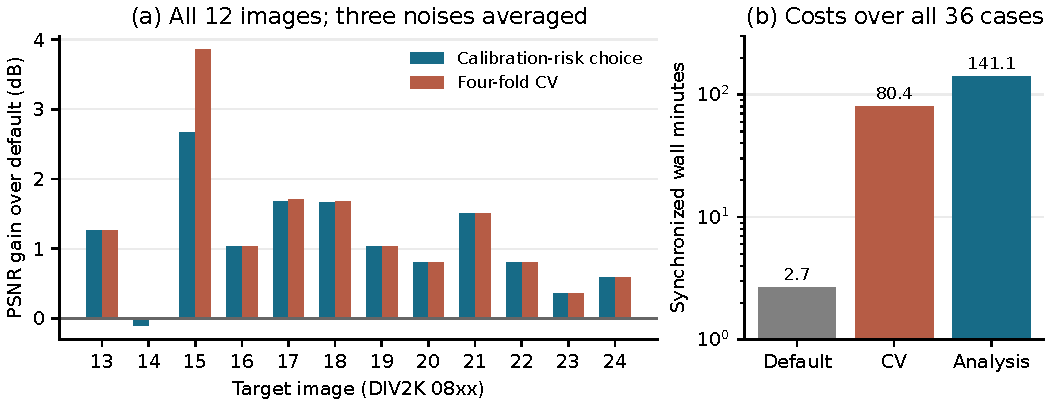
\includegraphics[width=\textwidth]{figures/guidance-results.pdf}
\caption{G2 complete-cohort gains and costs. (a) Every target image is
shown; averaging three noise settings does not create three independent
image replicates. (b) Synchronized wall time of common preparation,
selection and final fits on the same A800, on a log axis; this is not GPU
busy time. The analysis rule chooses power exponent 2.5 in all 36 cases,
so its gain does not establish instance-specific adaptation.}\label{fig:g2}
\end{figure*}

\paragraph{Results and counterexamples.} Analysis improves the default by
$1.105$ dB [.726, 1.504], with no $>1$ dB degradations, passing the
predeclared default-improvement gate (positive lower interval bound and
at most 5\% severe degradations). Its gains at the three noises are
$1.247,1.124,.945$ dB. CV improves the default by $1.217$ dB. The paired
analysis-minus-CV gain is $-.112$ dB [$-.313,-.002$], and analysis costs
1.76 times CV. The predeclared superiority-at-no-greater-cost gate fails
on both gain and cost. The frozen summarizer additionally requires zero
selection failures for that gate; there are none, so this extra restriction
does not change the conclusion \src{G2-result; G2-audit}.

Analysis chooses $1/f^{2.5}$ in 36/36 cases, whereas CV chooses exponents
2/2.5/3 in 3/27/6 cases. They hit the eight-candidate oracle in 25/36 and
34/36 cases respectively. Analysis loses to the default on image 0814 at
all three noises, worst $-.152$ dB; its largest oracle regret is 1.248 dB
on 0815 at .01 noise. A retrospective fixed-$1/f^{2.5}$ replay has
identical outputs to analysis, with common preparation and final fits
costing 194.6 s. This algebraic/cache identity is an interpretation of the
completed results, not an added confirmatory baseline or a new default
chosen before this test. The experiment does not isolate a benefit of
target-specific analytical selection \src{G2-audit}.

\paragraph{Full cost and practical reading.} Analysis and CV require
$5.065\times10^{12}$ and $3.222\times10^{12}$ interpolated points. Peak
recorded allocated memory is .488 GB. Calibration takes 3.0 s separately;
the actual resource ledger records 14,346.6 s of GPU-phase invocation wall
time, including the experiment's selection and oracle scoring, within the
24-hour budget. These timings depend on the shared-server load and are
not a benchmark of exclusive-device speed. Independent CPU audits reproduce
statistics and costs; all 78 cached chosen predictions were re-scored
from RGB pixels. Uncached candidate predictions were not retained, so
their oracle scores were audited from saved MSE and convergence records,
without an independent GP rerun. In this task, calibrated analysis finds
a better prior than the specified default, but frame-holdout CV adapts
more effectively and costs less. We therefore retain the analysis as a
conditional diagnostic, not a demonstrated cheap replacement for CV or
a neural-architecture selector \src{G2-audit}.
